\documentclass[conference]{IEEEtran}
\IEEEoverridecommandlockouts
% The preceding line is only needed to identify funding in the first footnote. If that is unneeded, please comment it out.
\usepackage{cite}
\usepackage{amsmath,amssymb,amsfonts}
%\usepackage{algorithmic}
\usepackage{graphicx}
\usepackage{textcomp}
\usepackage{xcolor}
\def\BibTeX{{\rm B\kern-.05em{\sc i\kern-.025em b}\kern-.08em
    T\kern-.1667em\lower.7ex\hbox{E}\kern-.125emX}}
    
% for algorithm
\usepackage{algorithm}
\usepackage{algpseudocode}
\newcommand{\vars}{\texttt}
\newcommand{\func}{\textrm}
\let\oldReturn\Return
\renewcommand{\Return}{\State\oldReturn}
\makeatletter
\renewcommand{\ALG@name}{Algoritma}
\makeatother
% for url
\usepackage{hyperref}

% for subfigure
\usepackage{subcaption}

% for multirow table
\usepackage{multirow}



\graphicspath{{assets/}{../assets/}}

\begin{document}

\title{Prediksi Arus Lalu Lintas secara \textit{Real-Time} menggunakan Kamera CCTV Jalan berbasis \textit{Deep Learning} dengan \textit{Long-Short Term Memory} (LSTM)\\
%{\footnotesize \textsuperscript{*}Note: Sub-titles are not captured in Xplore and
%should not be used}
%\thanks{Identify applicable funding agency here. If none, delete this.}
}

\author{\IEEEauthorblockN{Okta Fajar Suryani, Igi Ardiyanto, Addin Suwastono}
\IEEEauthorblockA{\textit{Departemen Teknik Elektro dan Teknologi Informasi} \\
\textit{Fakultas Teknik Universitas Gadjah Mada}\\
Yogyakarta, Indonesia \\
okta.fajar.s@mail.ugm.ac.id, \{igi; adyn\}@ugm.ac.id}
%\and
%\IEEEauthorblockN{2\textsuperscript{nd} Given Name Surname}
%\IEEEauthorblockA{\textit{dept. name of organization (of Aff.)} \\
%\textit{name of organization (of Aff.)}\\
%City, Country \\
%email address}
%\and
%\IEEEauthorblockN{3\textsuperscript{rd} Given Name Surname}
%\IEEEauthorblockA{\textit{dept. name of organization (of Aff.)} \\
%\textit{name of organization (of Aff.)}\\
%City, Country \\
%email address}
}

\maketitle

\begin{abstract}
Saat ini teknologi \textit{deep learning} telah banyak digunakan dalam berbagai bidang mulai dari pengolahan citra, pengenalan suara, klasifikasi bahkan deteksi suatu objek. Telah banyak jaringan deep learning yang dikembangkan. Untuk deteksi objek terdapat
YOLO (\textit{You Only Look Once}), SSD, dan Fast-RCNN sedangkan untuk data yang sifatnya sekuensial waktu terdapat LSTM, RNN dan GRU. 
	
Pada penelitian ini akan dibahas mengenai perancangan sebuah sistem agar dapat melakukan prediksi arus lalu lintas secara real-time menggunakan kamera CCTV jalan raya. Pendekatan yang dilakukan berbasis deep learning dengan menggunakan beberapa arsitektur yang telah ada.
Secara garis besar, proses perancangan sistem akan dibagi menjadi 3 bagian yaitu perancangan objek detektor menggunakan arsitektur YOLOV3 untuk diimplementasikan di CCTV, perancangan LSTM untuk prediksi jumlah kendaraan serta perancangan \textit{dashboard} untuk visualisasi sistem.
Objek detektor akan bertugas untuk melakukan deteksi jenis kendaraan, \textit{tracking} dan perhitungan jumlah kendaraan. LSTM bertugas untuk memprediksi arus lalu lintas berdasarkan data jumlah kendaraan yan telah dibuat oleh objek detektor. Untuk memberikan hasil yang optimal, kedua jaringan akan dilatih dan dievaluasi menggunakan metric nya masing-masing. 
Objek detektor akan dilatih menggunakan dataset sendiri pada \textit{framework} Darknet, dan dievaluasi menggunakan nilai precisions, recall, mAP dan F1-Score. 
Sedangkan LSTM akan dilatih dengan memvariasikan parameter jumlah lapisan LSTM, jumlah neuron tiap lapisan, jumlah data input, serta jumlah data output LSTM dan akan dievaluasi menggunakan data uji untuk mengetahui nilai \textit{Root Mean Squared Error} (RMSE) dan \textit{Mean Average Percentage Error} (MAPE). 
	
Data dari objek detektor dan LSTM akan ditampilkan jadi satu pada \textit{dashboard} sehingga informasi dari kedua model dapat dipahami lebih mudah.
\end{abstract}

\begin{IEEEkeywords}
\textit{Deep Learning}, \textit{You Only Look Once}, \textit{Long-Short Term Memory}, \textit{tracking}, precision, recall , F1-score, \textit{Root Mean Squared Error}, \textit{Mean Average Percentage Error }
\end{IEEEkeywords}

\section{Pendahuluan}
Kemacetan menjadi masalah serius di Indonesia. Berdasarkan survei yang dilakukan oleh Inrix, pada tahun 2017 Indonesia menempati peringkat ke 2 dunia dalam hal jumlah rata-rata waktu yang dihabiskan di jalan karena kemacetan. Selama tahun 2017 masyarakat Indonesia rata-rata menghabiskan waktu sia-sia di jalan (terjebak macet) sampai 51 jam \cite{Inrix2017Survei}. Sedangkan, berdasarkan index lalu lintas Indonesia menempati posisi ke 6 di Asia sebagai negara termacet dengan index 177.91 dari total index 216, index emisi $CO_2$ yang disebabkan kemacetan ini sebesar 6415.58 \cite{Numbeo2015Survei}. 
Di tahun yang sama, beberapa lembaga survei mencatat bahwa Jakarta menjadi kota termacet di Indonesia dengan level kemacetan mencapai 61\% \cite{TomTom2017Survei}. Kota kedua termacet di Indonesia adalah Bandung dengan rata-rata waktu yang dihabiskan di kemacetan sebesar 42,57 jam per tahun \cite{Inrix2017Survei}. Melihat kondisi seperti itu kemacetan membawa kerugian dari segi waktu maupun lingkungan.
Tak heran, saat ini informasi terkait arus lalu lintas yang akurat dan \textit{real time} sangat dibutuhkan untuk wisatawan atau travelers, sektor bisnis, dan lembaga pemerintah \cite{Zhang2008DynaCAS}.

Salah satu cara untuk menyediakan informasi arus lalu lintas yang akurat adalah dengan menggunakan metode prediksi. Dari sudut pandang otoritas transportasi, kemampuan untuk memprediksi pola lalu lintas merupakan persyaratan utama untuk efisiensi manajemen lalu lintas baik di perkotaan maupun di daerah sub-urban. Prediksi lalu lintas dapat digunakan untuk identifikasi awal terjadinya kemacetan sehingga memungkinkan otoritas lalu lintas mengambil tindakan pencegahan untuk mengurangi kemacetan
jalan \cite{Djahel2014SmartCity}. Dengan adanya prediksi arus lalu lintas, dapat diketahui bagaimana pengaruh arus saat ini terhadap kondisi jalan di periode waktu berikutnya sehingga dapat dibuat penjadwalan arus lalu lintas secara otomatis untuk suatu area kota \cite{Yuangfang2018TrafficPrediction}.

Melihat fakta bahwasannya data lalu lintas merupakan data dari waktu ke waktu yang memiliki suatu pola tertentu serta melihat potensi yang dimilki oleh \textit{deep learning} untuk pemrosesan gambar maupun video, tidak menutup kemungkinan bahwa dapat dibuat sebuah sistem prediksi lalu lintas cerdas berbasis deep learning dengan memanfaatkan peran kamera CCTV di jalan raya secara \textit{real time}. 
Menggunakan teknologi deep learning, kamera CCTV dapat difungsikan lebih jauh lagi misalnya untuk mengklasifikasikan jenis kendaraan, menghitung jumlah kendaraan, serta memberikan prediksi arus lalu lintas untuk jam atau hari tertentu. Sehingga berdasarkan hasil analisa tersebut dapat disusun suatu strategi optimalisasi lalu lintas yang lebih efektif, efisien dan dapat mengurangi kemacetan. 
Tentu saja hal ini akan sangat membantu dan membawa dampak yang besar. Dengan berkurangnya tingkat kemacetan karena arus lalu lintas dapat diprediksi sebelumnya, membuat orang-orang dapat menghewat waktunya lebih banyak, tidak terbuang sia-sia di jalanan karena kemacetan panjang, dan dapat melakukan berbagai hal yang lebih produktif. 
Selain itu distribusi barang dan jasa bisa menjadi lebih cepat dimana hal ini sangat berpengaruh terhadap perekonomian negara. 

\section{Tinjauan Pustaka}

\subsection{Deteksi, \textit{tracking} dan perhitungan jumlah kendaraan}

Berbagai macam pendekatan telah dilakukan untuk mengembangkan sistem yang dapat mendeteksi, menghitung dan mengklasifikasikan jenis kendaraan sehingga dapat digunakan untuk pengawasan lalu lintas dalam sistem transportasi cerdas.

Lei, M. melakukan penelitian seputar perhitungan jumlah kendaraan berbasis video. Dalam penelitian tersebut, digunakan metode \textit{Adaptive background estimation} dan \textit{Gaussian shadow elimination}. Seperti kebanyakan metode pengolahan citra konvensional, kelemahan utama terletak pada pengaruh pencahayaan. Dalam penelitian tersebut akurasi perhitungan
sangat bergantung pada kemampuan untuk menghilangkan efek bayangan karena pengaruh pencahayaan. Selain itu sistem yang dikembangkan oleh \cite{Lei2018VehicleCounting} belum mampu mengklasifikasikan kendaraan dengan bagus.
Pada \cite{Sheeraz2018VehicleDetection}, juga dilakukan penelitian untuk klasifikasi dan perhitungan jumlah kendaraan berbasis video dengan membandingan performa metode pengolahan citra biasa dengan metode \textit{machine learning} sederhana. Dalam penelitian \cite{Sheeraz2018VehicleDetection}, perhitungan jumlah kendaraan dilakukan dengan mensubtraksi background menggunakan metode \textit{Gaussian Mixture Model} (GMM) sedangkan untuk klasfikasi menggunakan \textit{Contour Comparison} (CC) dan kombinasi antara \textit{Bag of Features}
(BoF) dengan \textit{Support Vector Machine} (SVM). Hasil penelitian menunjukan bahwa CC memiliki akurasi klasifikasi lebih tinggi daripada BoF \& SVM dengan selisih tidak terlalu jauh. 
Meskipun demikian, hal ini menunjukkan bahwa metode klasifikasi dan perhitungan jumlah kendaraan berbasis algoritma \textit{learning} memiliki prospek yang menjanjikan.
Salah satu penelitian dalam bidang deteksi, \textit{tracking} dan perhitungan jumlah kendaraan yang berbasis \textit{deep learning} adalah penelitian \cite{Chaucan2019CNN}. Pada penelitian ini digunakan model YOLO yang telah dilatih ulang untuk melakukan deteksi dan klasifikasi. Dataset yang digunakan berasal dari data Delhi-NCR. Hasil penelitian ini menunjukan bahwa menggunakan model \textit{deep learning} untuk klasifikasi dan deteksi memberikan akurasi yang tinggi.

\subsection{Prediksi arus lalu lintas}

Informasi arus lalu lintas yang akurat sangat penting untuk manajemen dan pengembangan sistem transportasi cerdas. Termasuk salah satunya adalah prediksi arus lalu lintas. Oleh karenanya, berbagai penelitian telah dilakukan untuk memberikan hasil prediksi arus lalu lintas yang akurat.
Penelitian yang dilakukan oleh \cite{LSTM_2} menggunakan model encoder-decoder \textit{Long-Short Term Memory} (LSTM). Data yang digunakan berasal dari Caltrans Performance Measurement System (PeMS). Model yang telah dibuat dibandingkan dengan beberapa model lain seperti Random Walk (RW), Support Vector Regression (SVR) dan Wavelet Neural Network (WNN). 
Penelitian serupa dilakukan oleh \cite{LSTM_1}. Penelitian tersebut juga menggunakan LSTM untuk melakukan prediksi arus lalu lintas kapal di jalur air pedalaman sungai Yangtze Wuhan, China secara \textit{short-term} dan \textit{long-term}. Data yang digunakan berasal dari Changjiang Maritime Safety Administration. Penelitian ini juga membandingkan performa LSTM dengan beberapa model lain yaitu GRU, DBNs, Linear Regression (LR) dan ARIMA.
Kedua penelitian \cite{LSTM_1} dan \cite{LSTM_2} memberikan hasil yang menunjukkan bahwa model LSTM memberikan hasil yang lebih baik untuk prediksi secara \textit{short-term} maupun \textit{long-term}

\subsection{YOLO (\textit{You Only Look Once}) V3}

\textit{You Only Look Once} (YOLO) merupakan suatu metode pendekatan yang bertujuan untuk deteksi objek. YOLO melihat deteksi objek sebagai suatu masalah regresi dari \textit{bounding box} dan
probabilitas kelas yang terpisah secara spasial. YOLO merupakan \textit{neural network} yang memprediksi \textit{bounding box} dan \textit{class probability} dari gambar utuh secara langsung dalam satu kali
evaluasi. Oleh karena deteksi YOLO menggunakan \textit{single network}, maka optimasi performa deteksi dapat dilakukan langsung secara end-to-end \cite{YoloV1}.

Secara arsitekturnya, YOLO hanya menggunakan lapisan konvolusi sehingga menjadikannya sebuah jaringan konvolusi penuh (FCN). Pada YOLOV3 terdapat 75 lapisan konvolusi dengan \textit{skip connection} dan lapisan upsampling.
YOLOv3 menggunakan stride 2 untuk \textit{downsample} fitur map serta tidak menggunakan lapisan \textit{pooling} untuk mencegah hilangnya informasi dari fitur tingkat rendah. Pada YOLOV3 setiap \textit{bounding box} memiliki atribut array ukuran \textbf{(5 + C)} dimana array ini mengandung informasi
mengenai koordinat titik tengah, ukuran dimensi, skor objektivitas, dan $C$ skor kelas.

YOLOV3 mendeteksi suatu objek dengan cara membagi gambar input kedalam grid sebanyak ukuran fitur map. Kemudian masing-masing grid akan memprediksi \textit{bounding box} sebanyak 3 buah.
Kemudian jaringan akan mencari grid yang berpotensi memiiliki koordinat titik tengah suatu objek pada gambar input. Grid-grid tersebutlah yang kemudian akan bertanggung jawab untuk melakukan prediksi \textit{bounding box} untuk objek \cite{YoloV3}.

Sebagai contoh, misalkan suatu gambar input berukuran 416x416 dan stride pada lapisan deteksi bernilai 32, maka fitur map akan memiliki dimensi 13x13. Selanjutnya gambar input akan dibagi menjadi 13 grid seperti pada gambar \ref{grid_YOLO}.
\begin{figure}
	\centering
	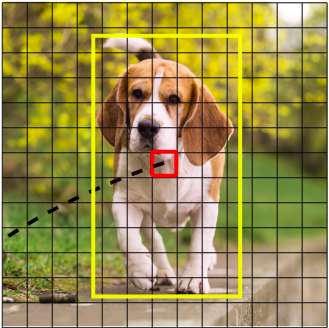
\includegraphics[scale=0.5]{grid_input}
	\caption{Gambar input dibagi kedalam grid sesuai ukuran fitur map}
	\label{grid_YOLO}
\end{figure}
Berdasarkan gambar \ref{grid_YOLO}, grid yang berpotensi memiliki koordinat titik tengah objek adalah grid merah (baris dan kolom ke-7). Berarti, grid inilah yang bertugas untuk memprediksi \textit{bounding box} dari objek (anjing). 

YOLO memprediksi titik tengah \textit{bounding box} dengan mencari offset relatif terhadap grid pojok kiri atas dari grid yang bertugas untuk memprediksi \cite{YoloV2}. Pada contoh diatas, grid yang digunakan sebagai acuan adalah grid (6,6).
Persamaan untuk mencari \textit{bounding box}:
\begin{equation} \label{bx_bb}
	b_{x} = \sigma(t_{x}) + c_x
   \end{equation}
\begin{equation} \label{by_bb}
	b_{y} = \sigma(t_{y}) + c_y
\end{equation}
\begin{equation} \label{bw_bb}
	b_{w} = p_{w}e^{t_w}
\end{equation}
\begin{equation} \label{bh_bb}
	b_{h} = p_{h}e^{t_h}
\end{equation}
$b_x$, $b_y$: koordinat titik tengah pada gambar input, $b_w$, $b_h$: lebar dan tinggi hasil prediksi, $t_x$, $t_y$: koordinat titik tengah terhadap grid, $t_w$, $t_h$: lebar dan tinggi terhadap grid, $c_x$, $c_y$: grid acuan (pojok kiri atas), pada contoh diatas grid (6,6). Sedangkan $p_h$, $p_w$: dimensi anchor box yang digunakan. 
$t_x$, $t_y$ dilewatkan fungsi sigmoid agar nilainya berada diantara 0 dan 1. Hal ini agar koordinat titik tengah hasil prediksi tidak keluar dari grid yang bertugas melakukan prediksi, dalam contoh diatas yaitu grid (7,7)

Skor kelas menunjukan probabilitas objek yang terdeteksi milik kelas tertentu. Pada YOLO, dan YOLOV2 skor kelas menggunakan softmax, sedangkan pada YOLOV3 menggunkan sigmoid.
Skor kelas yang dihitung menggunakan softmax mengasumsikan bahwa kelas-kelas tersebut saling eksklusif. Dengan kata lain, jika suatu objek telah terdeteksi milik satu kelas, maka dijamin tidak bisa milik kelas lain. 
Namun, asumsi ini kurang cocok digunakan ketika memiliki 2 atau lebih kelas dengan fitur yang hampir mirip, sebagai contoh kelas wanita dan orang. Oleh karena inilah, YOLOV3 mengunakan sigmoid untuk skor kelas \cite{YoloV3}.

\subsection{Prediksi menggunakan LSTM}

Sebagai contoh dalam kasus prediksi arus lalu lintas, misalnya runtun nilai input adalah $X = (x_{1},x_{2},...,x_{T})$ , hidden vektor yang terhitung adalah $H = (h_{1},h_{2},...,h_{T})$ dan runtun yang akan diprediksi adalah $Y = (y_{1},y_{2},...,y_{T})$. 
Proses pembaruan setiap timestep $t$ pada lapisan sel memori LSTM dideskripsikan sebagai berikut:
\begin{equation} \label{input_gate}
 i_{t} = \sigma(W_{i}x_{t} + U_{i}c_{t-1}+b_{i})
\end{equation}
\begin{equation} \label{forget_gate}
	f_{t} = \sigma(W_{f}x_{t} + U_{f}c_{t-1}+b_{f})
\end{equation}
\begin{equation} \label{cell_state}
	c_{t} = f_{t}\circ c_{t-1} + i_{t}\circ g(W_{c}x_{t}+b_{c})
\end{equation}
\begin{equation} \label{output_gate}
	o_{t} = \sigma(W_{o}x_{t} + U_{o}c_{t-1}+b_{o})
\end{equation}
\begin{equation} \label{hidden_state}
	h_{t} = o_{t} \circ \sigma_{h}(c_{t})
\end{equation}
\begin{equation} \label{result_gate}
	y_{t} = \phi(W_{y}h_{t} + b_{y})
\end{equation}

Pada persamaan diatas $W_{i}$,$W_{f}$,$W_{c}$, $W_{o}$, $W_{y}$, $U_{i}$,$U_{f}$, $U_{o}$ adalah matiks bobot. Sedangkan $b_{i}$,$b_{f}$, $b_{c}$, $b_{o}$, $b_{y}$ adalah vektor bias.
$\circ$ adalah perkalian \textit{element-wise} dari vektor. $\sigma$, $g$, $\phi$ adalah fungsi aktivasi.

\section{Perancangan Sistem}
Pada bab ini, akan dibahas mengenai pendekatan yang digunakan untuk memecahkan permasalah terkait deteksi objek dan prediksi arus lalu lintas menggunakan LSTM. Untuk permasalahan yang terkait deteksi objek meliputi deteksi objek itu sendiri, \textit{tracking} dan perhitungan jumlah kendaraan. Sedangkan
untuk masalah prediksi menggunakan \textit{Long-Short Term Memory} meliputi pengolahan data, proses pelatihan dan pengujian.

Keseluruhan proses untuk mendapatkan model baik untuk deteksi objek maupun prediksi menggunakan LSTM dijabarkan pada gambar \ref{get_model_scheme}.
\begin{figure}[htp]
	\centering
	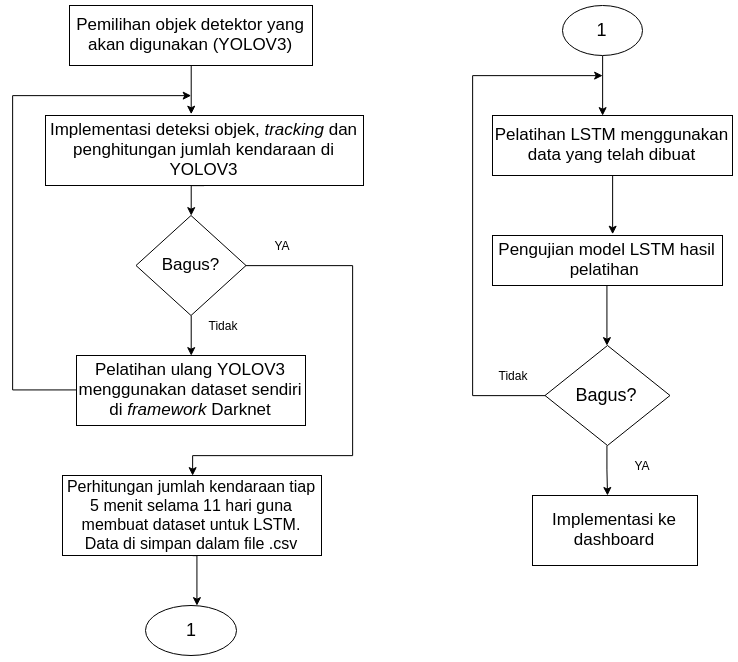
\includegraphics[scale=0.4]{Get_Model_Scheme}
	\caption{Keseluruhan proses untuk mendapatkan model terbaik}
	\label{get_model_scheme}
\end{figure}

\subsection{Deteksi objek}
Berdasarkan gambar \ref{get_model_scheme}, proses pertama yang dilakukan adalah pemilihan jaringan objek detektor. Seperti yang telah disebutkan pada bagian dasar teori, terdapat beberapa jaringan objek detektor yang telah dikembangkan oleh ilmuan. 
Gambar \ref{yolo_comparison} menunjukan perbandingan performa dari beberapa jaringan objek detektor yang ada saat ini.
\begin{figure}
	\centering
	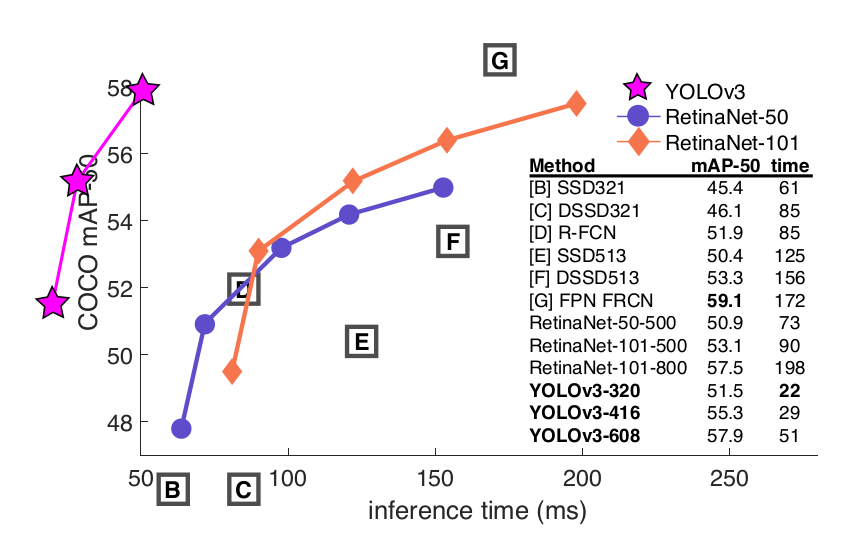
\includegraphics[scale=0.4]{YOLO_Comparison}
	\caption{Perbedaan performa beberapa network objek detektor}
	\label{yolo_comparison}
\end{figure}

Berdasarkan perbandingan tersebut, akhirnya dipilih YOLOV3-416 sebagai objek detektor pada penelitian ini. Pertimbangan ini didasari performa YOLOV3-416 yang memiliki mAP-50 cukup tinggi dengan waktu \textit{inference} yang cukup cepat. 
mAP-50 yang cukup tinggi diperlukan agar deteksi objek yang dihasilkan baik dan akurat, waktu \textit{inference} yang cukup cepat diperlukan agar deteksi yang diberikan dapat \textit{real time}. 416 menunjukan ukuran gambar input. Ukuran gambar yang tidak terlalu besar akan mempercepat proses komputasi di GPU.

Setelah YOLOV3 diuji, ditemukan bahwa meskipun YOLOV3-416 memiliki performa yang bagus dibandingkan objek detektor lainnya, objek detektor ini memberikan hasil yang kurang optimal apabila diterapkan untuk deteksi kendaraan pada lalu lintas di Indonesia secara langsung dari CCTV. Hasil deteksi YOLOV3-416 original pada lalu lintas Indonesia ditunjukkan oleh gambar \ref{yoloV3_ori}

\begin{figure}[htp]
	\centering
	\includegraphics[scale=0.5]{yoloV3}
	\caption{Hasil deteksi kendaraan oleh YOLOV3-416 pada lalu lintas Indonesia}
	\label{yoloV3_ori}
\end{figure}
Berdasarkan gambar \ref{yoloV3_ori}, YOLOV3-416 mengalami kesulitan untuk mendeteksi objek sepeda motor secara benar.
Dikarenakan hasil deteksi akan digunakan pada proses perhitungan jumlah kendaraan, maka dibutuhkan objek detektor yang mampu medeteksi kendaraan degan benar terutama mobil dan sepeda motor yang menjadi kendaraan utama di lalu lintas Indonesia.

Oleh karena itu seperti gambar \ref{get_model_scheme} dilakukan proses ketiga yaitu pelatihan ulang YOLOV3. Untuk melakukan pelatihan ulang maka diperlukan dataset dari kondisi permasalahan sebenarnya. Proses pengambilan dataset dilakukan dengan cara mengumpulkan gambar-gambar yang berkaitan dengan kondisi lalu lintas di Indonesia yang dilihat dari CCTV. Gambar-gambar tersebut diperoleh dari layanan \textit{live streaming} ATCS di beberapa kota. 
Setelah data terkumpul, maka dilakuakan proses pelabelan (\textit{hand labeling}) untuk membuat \textit{groundtruth}. Untuk mempercepat proses pelabelan dataset maka digunakan aplikasi LabelImg \cite{LabelImg}. LabelImg merupakan tools yang \textit{open source} di GitHub. Berikutnya yang perlu dilakukan adalah mengatur parameter pelatihan seperti inisiasi \textit{learning rate}, iterasi maksimum, iterasi awal mulai penerapan \textit{adaptive learning rate}, \textit{batch size}, serta anchor box. Semua parameter training diatur dan disimpan dalam file konfigurasi .cfg dimana file ini akan 
dipanggil saat proses pelatihan. Darknet telah menyediakan fasilitas untuk menghitung metric evaluasi model antara lain \textit{True Positive (TP), False Positive (FP), False Negative (FN), precision, recall, F1-score, IoU}, dan \textit{Mean Average Precision} (mAP).

\subsubsection{\textit{Tracking} dan Perhitungan Jumlah Kendaraan}
Tracker yang digunakan pada penelitian ini adalah \textit{Simple Online and Real-time Tracking} (SORT) \cite{SORT}. Pada SORT, ketika terdapat objek yang terdeteksi, \textit{bounding box} dari objek akan digunakan untuk menentukan state target. Estimasi geometri \textit{bounding box} untuk target dilakukan dengan memprediksi lokasi berikutnya pada frame saat ini. Prediksi lokasi ini berdasarkan pada komponen kecepatan yang diselesaikan oleh Kalman Filter \cite{Kalman}.
\begin{algorithm}[htp]
	\begin{algorithmic}[1]
		%\State $boxes.append([x, y, w, h])$ 
		%\State $memory[indexIDs[-1]] \leftarrow boxes[-1]$
		\If {$len(boxes) > 0$}
			\State $i \leftarrow 0$
			\For { $box \in boxes$ }
				\State $(x, y) \leftarrow (int(box[0]), int(box[1]))$
				\State $(w, h) \leftarrow (int(box[2]), int(box[3]))$
				\If {$indexIDs[i] \in previous$}
					\State $previous_box \leftarrow previous[indexIDs[i]]$
					\State $(x2, y2) \leftarrow (int(previous_box[0]), int(previous_box[1]))$
					\State $(w2, h2) \leftarrow (int(previous_box[2]), int(previous_box[3]))$
					\State $p0 \leftarrow (int(x + (w-x)/2), int(y + (h-y)/2))$
					\State $p1 \leftarrow (int(x2 + (w2-x2)/2), int(y2 + (h2-y2)/2))$
					\State $buat garis (p0, p1)$
					\If {$intersect(p0, p1, line[0], line[1])$}
						\State $counter += 1$
					\EndIf
				\EndIf
				\State $i \leftarrow i+1$
			\EndFor
		\EndIf
	\end{algorithmic}
	\caption{Proses perhitungan jumlah kendaraan}
	\label{counting_ob}
\end{algorithm}

Berdasarkan algoritma \ref{counting_ob} diketahui bahwa agar suatu objek dapat terhitung maka objek tersebut harus melewati garis acuan perhitungan dan garis pada objek harus bersinggungan dengan garis acuan tersebut. 
Untuk menentukan apakah dua buah garis bersinggungan atau tidak, dilakukan dengan menentukan formasi 3 dari 4 titik dua garis yang bersinggungan terlebih dahulu kemudian membawa konsep formasi ini untuk pengambilan keputusan.

Formasi acuan yang digunakan adalah formasi \textit{counterclockwise} (ccw). Misalkan terdapat titik A, B, dan C seperti pada gambar \ref{ccw_img}. Tiga titik tersebut dapat dikatakan memiliki formasi ccw jika \textbf{\textit{gradien garis AC > gradien garis AB}}
sehingga harus memenuhi persamaan \ref{ccw_eq}.
\begin{equation} \label{ccw_eq}
	(C_y - A_y)*(B_x - A_x) > (B_y - A_y)*(C_x - A_x)
\end{equation}

\begin{figure}[htp]
	\centering
	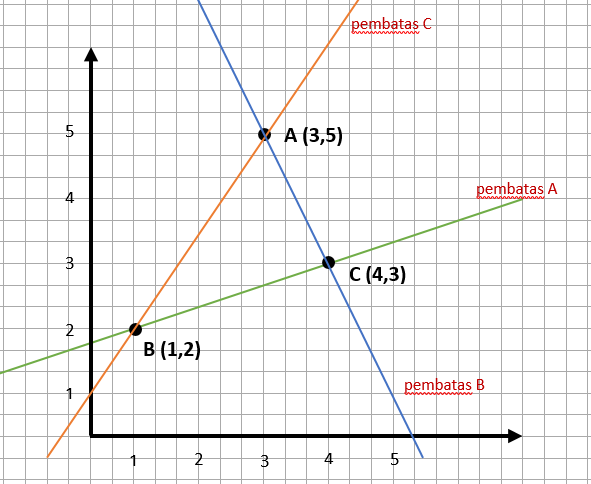
\includegraphics[scale=0.5]{CCW}
	\caption{Ilustrasi formasi 3 titik secara \textit{counterclockwise}}
	\label{ccw_img}
\end{figure}

Berikutnya, konsep formasi akan digunakan untuk menentukan keputusan apakah dua buah garis bersinggungan atau tidak. Garis AB dan garis CD akan bersinggungan \textbf{\textit{jika dan hanya jika titik C dan D dipisahkan oleh garis AB}}.
Jika titik A dan B dipisahkan oleh garis CD, maka ACD dan BCD, ADC dan BDC, CAD dan CBD, DAC dan DBC memiliki orientasi yang berbeda. Begitu juga apabila titik C dan D dipisahkan oleh garis AB maka ACB dan ADB, CAB dan DAB, CBA dan DBA, BAC dan BAD memiliki orientasi yang berbeda. Dari berbagai kombinasi tersebut cukup diambil masing-masing satu saja.
Jika dirumuskan secara matematis menjadi persamaan \ref{intersect_eq}.
\begin{equation} \label{intersect_eq}
	ccw(A,C,D) =! ccw(B,C,D) \hspace{5mm} and \hspace{5mm} ccw(A,B,D) =! ccw(A,B,C)
\end{equation}
Sehingga apabila dua buah garis saling bersingungan persamaan \ref{intersect_eq} akan memberikan nilai benar.

\subsection{Prediksi Arus Lalu Lintas menggunakan LSTM}
Proses pertama yang dilakukan adalah pelatihan untuk memperoleh model LSTM. Alur tahapan pelatihan dijabarkan seperti pada gambar \ref{lstm_training}.
\begin{figure}
	\centering
	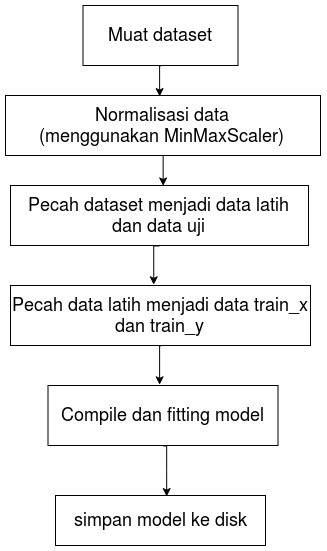
\includegraphics[scale=0.5]{Training_lstm}
	\caption{Tahapan pada proses pelatihan (\textit{training})}
	\label{lstm_training}
\end{figure}

Pada proses ini, akan dilakukan pelatihan dengan memvariasikan beberapa parameter jaringan LSTM antara lain jumlah runtun data input dan output, jumlah lapisan LSTM yang digunakan serta jumlah neuron per lapisan LSTM. 
Masing-masing model ini akan masuk tahap pengujian untuk dievaluasi. Alur tahapan pengujian dijabarkan seperti pada gambar \ref{lstm_testing}.
\begin{figure}[t]
	\centering
	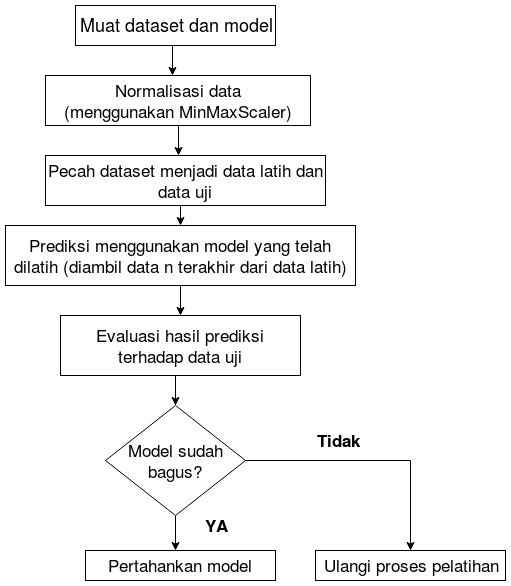
\includegraphics[scale=0.5]{Testing_lstm}
	\caption{Tahapan pada proses pengujian (\textit{testing})}
	\label{lstm_testing}
\end{figure}

Untuk mendapatkan hasil prediksi, dilakukan dengan mengambil sebanyak $n\_input$ data dari data latih. Data ini akan menjadi input untuk LSTM. LSTM pada Keras membutuhkan input array 3 dimensi yang memiliki bentuk ($N, W, F$) dimana $N$: jumlah runtun, $W$: panjang runtun data input, dan $F$: adalah jumlah fitur setiap runtun sehingga data input harus di\textit{reshape} menjadi bentuk seperti yang diperbolehkan.
Proses tersebut dilakukan di dalam sebuah perulangan. Tiap iterasi akan menghasilkan array hasil prediksi. Selain itu pada setiap akhir iterasi, data input akan digabung dengan data uji (sesuai indeks iterasi). Proses lebih jelas dijabarkan pada algoritma \ref{test_LSTM}.
\begin{algorithm}[htp]
	\begin{algorithmic}[1]
	\Function{get_prediction}{$train, test, n\_input$}
		\State $model \leftarrow get\_model()$
		\State $data\_input \leftarrow array(train)$
		\State $data\_input \leftarrow data\_input.reshape$
		\State $prediction \leftarrow list()$
		\For { $i \in range(len(test))$ }
			\State $data \leftarrow data\_input$
			\State $input\_x \leftarrow data[-n\_input:,0]$
			\State $input\_x \leftarrow input\_x.reshape((1, len(input\_x), 1))$
			\State $yhat \leftarrow model.predict(input\_x, verbose=0)$
			\State $yhat\_sequence \leftarrow yhat[0]$
			\State $predictions.append(yhat\_sequence)$
			\State $test\_append = test[i, :]$
			\State $data\_input \leftarrow np.append(data\_input, test\_append, axis=0)$
		\EndFor
	\EndFunction
	\end{algorithmic}
	\caption{Proses prediksi menggunakan LSTM}
	\label{test_LSTM}
\end{algorithm}

Setelah model terbaik dari objek detektor dan model LSTM diperoleh, model ini akan digunakan pada proses implementasi sistem. Proses implementasi serta pengiriman dan penerimaan data dari satu proses ke proses yang lain dijabarkan pada gambar \ref{implementasi_sistem}.

\begin{figure}[htp]
	\centering
	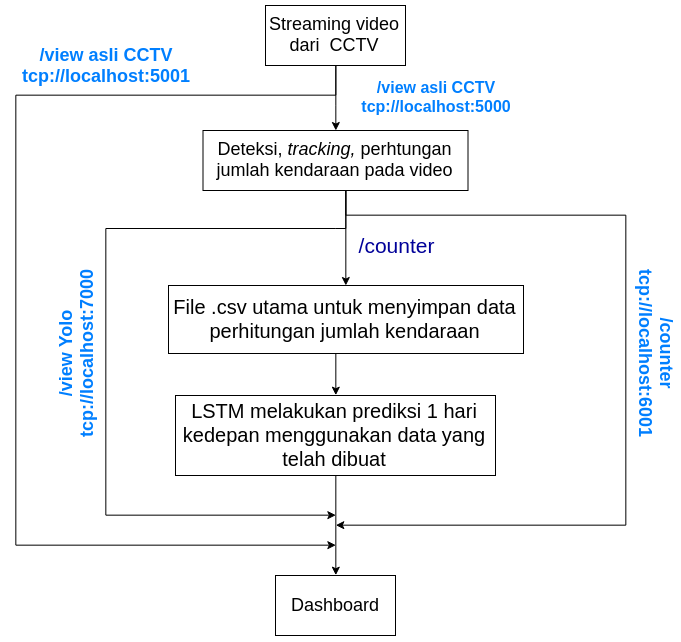
\includegraphics[scale=0.5]{Sistem_all}
	\caption{Urutan proses implementasi menggunakan model yang telah diperoleh}
	\label{implementasi_sistem}
\end{figure}

\section{Hasil dan Pembahasan}
\subsection{Deteksi Objek}
Jumlah total dataset adalah 1856 gambar dengan pembagian data pelatihan sebanyak 1688 gambar dan data uji sebanyak 168 gambar.
Pada proses pembuatan dataset ini dilakukan teknik augmentasi variasi tingkat saturasi dan kecerahan gambar. Teknik augmentasi seperti rotasi dan \textit{flip} tidak digunakan karena kondisi lalu lintas indonesia yang sangat padat sehingga 
terdapat banyak kendaraan yang memiliki daerah tumpang tindih.

Setting untuk proses pelatihan dilakukan pada file \textit{configuration} dimana Darknet akan membaca file ini. Untuk pelatihan pada penelitian ini menggunakan jumlah perulangan 12000 dengan 6 kelas sehingga setiap kelas akan dilatih sebanyak 2000 perulangan. 
\textit{Adaptive learning rate} juga diterapkan ketika perulangan telah mencapai 70\% dan 90\% dari total perulangan. Hal ini dilakukan agar informasi yang dilatih oleh jaringan semakin detail. Grafik pelatihan ditunjukan oleh gambar \ref{train_darknet}. Berdasarkan gambar tersebut, metric yang diamati selama pelatihan adalah mAP (\textit{mean average precision}) dan loss pelatihan.
\begin{figure}[htp]
	\centering
	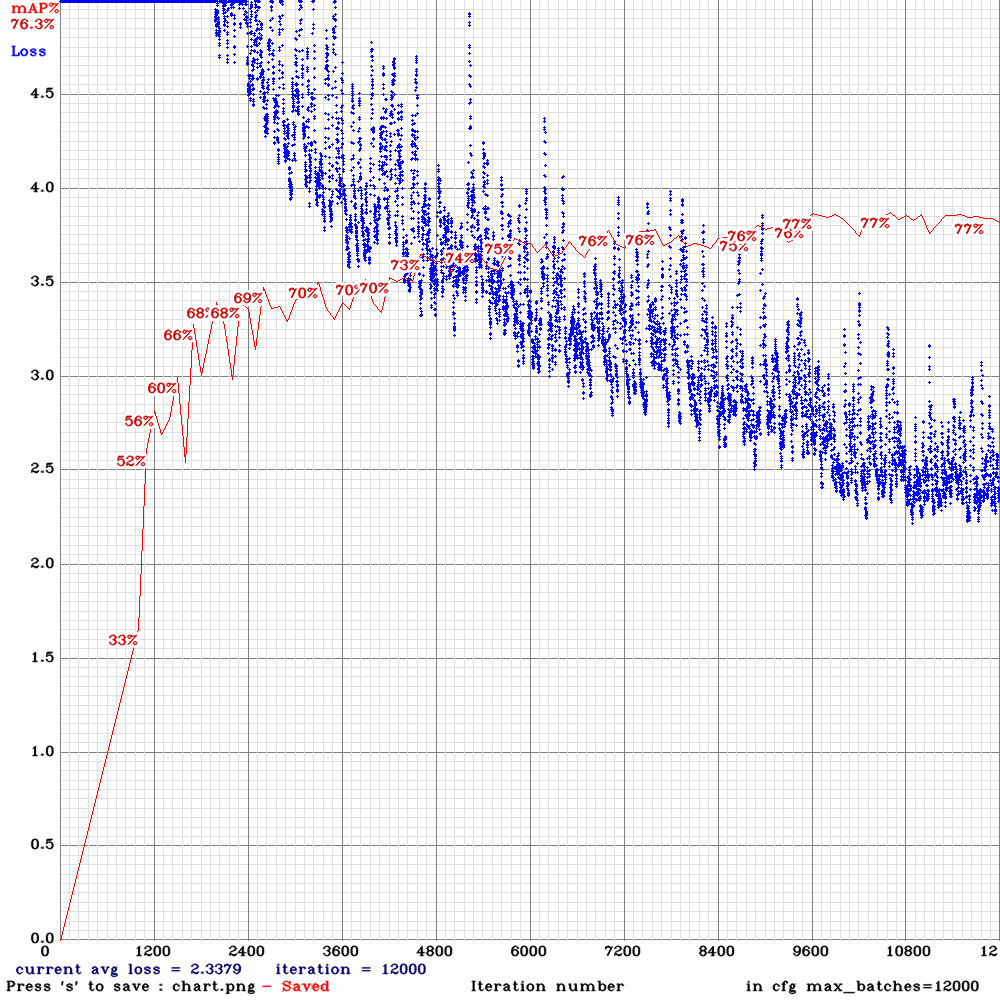
\includegraphics[scale=0.25]{new_full_dataset}
	\caption{Grafik proses pelatihan}
	\label{train_darknet}
\end{figure}
Dari gambar juga dapat diketahui bahwa model yang telah dilatih tidak mengalami \textit{overfitting}. Hal ini dapat dilihat dari grafik mAP (merah) yang terus mengalami kenaikan sedangkan grafik loss pelatihan (biru) mengalami penurunan.
Hasil pelatihan model pada masing-masing kelas dapat dilihat pada tabel \ref{Tabel_training}.
\begin{table}[htp]
\centering
\begin{tabular}{ cccccc }
	\hline 
	Kelas Id & Nama Kelas & AP & TP & FP\\
	\hline
	0& Person & 89.3\% & 10 & 2\\
	1 & Car & 94.93\% & 1624 & 171\\
	2 & Motorbike& 89.93\% &1092& 212 \\
	3 & Bus & 84.73\% & 27& 5 \\
	4 & Truck & 94.60\% & 191 & 27\\
	5 & Bicycle & 0.00\% &0 & 0 \\
\end{tabular}
\caption{Hasil pelatihan untuk tiap kelas}
\label{Tabel_training}
\end{table} 

Berdasarkan tabel tersebut dapat dilihat bahwa kelas yang memiliki \textit{average precision} terbesar adalah mobil, truck dan sepeda motor. Hal ini dikarenakan data latih atau kondisi lalu lintas Indonesia didominasi oleh tiga kelas tersebut, terutama mobil dan motor. 
Dari tabel \ref{Tabel_training} juga diketahui bahwa Total TP = 2944, Total FP = 417, dengan IoU = 68.22\% memberikan Total FN = 401. Maka dapat dicari nilai precision, recall dan F1-score nya berdasarkan persamaan \ref{Recall}, \ref{Precision}, \ref{F1_score}.
\begin{equation} \label{Precision}
	Precision = \frac{TP}{TP+FP} = \frac{2944}{2944+417} = 0.8759
\end{equation}

\begin{equation} \label{Recall}
	Recall = \frac{TP}{TP+FN} = \frac{2944}{2944+401} = 0.88
\end{equation}

\begin{equation} \label{F1_score}
	F1-score = 2*\frac{Precision * Recall}{Precision + Recall} = 2*\frac{0.88 * 0.8759}{0.88 + 0.8759} = 0.8779
\end{equation}

\subsection{Perhitungan jumlah kendaraan}

Hasil perhitungan jumlah kendaraan oleh model yang telah dilatih kemudian dibandingkan dengan data acuan untuk mengetahui besaran error yang diberikan. Dalam penelitian ini, data acuan merupakan data hasil pengamatan secara langsung oleh pengamat yang diambil dari sampel 15 menit.
Metode mendapatkan data acuan ini dilakukan karena ATCS kota Semarang belum memiliki database yang berisi jumlah kendaraan tiap 5 menit. Untuk memberikan informasi yang lebih valid, pembuatan data acuan dilakukan oleh dua pengamat.
Hasil perbandingan antara perhitungan sistem dengan pengamat dapat dilihat pada tabel \ref{Count_result}. 
\begin{table}[htp]
\centering
\begin{tabular}{|c|c|c|c|}
	\hline 
	\multirow{2}{*}{\textbf{5 menit ke-}} & \multicolumn{2}{c|}{\textbf{Grountruth}} &  \multirow{2}{*}{\textbf{Hasil perhitungan sistem}}\\ \cline{2-3}
	& Orang 1& Orang 2 &\\
	\hline
	1& 212 & 206 & 184\\
	2 & 270 & 278 & 254\\
	3 & 200 & 192 & 177\\
	4 & 227 & 235 & 204 \\
	5 & 223 & 232 & 202 \\
	6 & 248 & 241 & 235 \\
	7 & 232 & 208 & 217 \\
	8 & 235 & 241 & 213 \\
	9 & 269 & 273 & 248 \\
	10 & 265 & 271 & 243 \\
	11 & 229 & 235 & 206 \\
	\hline
\end{tabular}
\caption{Perbandingan hasil perhitungan sistem dengan \textit{groundtruth}}
\label{Count_result}
\end{table} 
Berdasarkan tabel \ref{Count_result} diketahui bahwa rata-rata error perhitungan oleh sistem tiap 5 menit sebesar 20 kendaraan.

\subsection{Prediksi arus lalu lintas menggunakan LSTM}
Berdasarkan skema pengambilan data jumlah kendaraan diatas, diperoleh data dengan jumlah 1430 data untuk 11 hari sehingga per hari terdapat 130 data.
Proses pengolahan data yang dilakukan yaitu membagi data menjadi data latih dan data uji. Pada penelitian ini data latih sebanyak 1170 data (9 hari) dan data uji sebanyak 260 data (2 hari)
Untuk proses pelatihan sendiri akan memvariasikan beberapa parameter yaitu jumlah lapisan LSTM, jumlah neuron tiap lapisan, jumlah data input, serta jumlah data output LSTM. 
Jumlah lapisan yang akan digunakan yaitu 1,2, dan 3 LSTM, jumlah neuron yang digunakan 50 dan 100, jumlah data input yang digunakan adalah 130, 260 dan 390, sedangkan jumlah output yang digunakan adalah 130, 65, dan 1. Masing-masing 
variasi akan diamati nilai RMSE, dan MAPE nya. Variasi yang memberikan nilai RMSE dan MAPE terendah akan dipakai untuk implementasi di dashboard.

Setelah melakukan proses pelatihan diperoleh model sebanyak variasi. Nilai RMSE dan MAPE masing-masing model dapat dilihat pada tabel \ref{1LSTM_result}, \ref{2LSTM_result}, dan \ref{3LSTM_result}.
\begin{table}[htp]
\centering
\begin{tabular}{|c|c|c|c|c|c|}
	\hline 
	\multirow{3}{*}{\textbf{Input LSTM}} & \multirow{3}{*}{\textbf{Output LSTM}} & \multicolumn{4}{c|}{\textbf{1 LSTM}} \\ \cline{3-6}
	&  & \multicolumn{2}{c|}{50}& \multicolumn{2}{c|}{100} \\ \cline{3-6}
	& & RMSE & MAPE& RMSE & MAPE\\
	\hline
	\multirow{3}{*}{130} & 130 & 30.34& 11.316\%& 28.153 & 10.878\%\\
	& 65 & 31.782 & 11.628\% & 26.919 & 11.353\% \\
	& 1 & 28.468 & 11.491\% & 27.669 & 11.614\% \\
	\hline
	\multirow{3}{*}{260} & 130 & 29.142 & 11.67\%  & 27.716 & 10.864\%\\
	& 65 & 29.784 & 11.458\% & 29.830 & 12.022\%\\
	& 1 & 28.267 & 11.389\% & 27.883 & 11.440\% \\
	\hline
	\multirow{3}{*}{390} & 130 & 32.301 & 12.446\% & 30.567 & 11.416\% \\
	& 65 & 32.015 & 12.541\% & 30.664 & 12.220\% \\
	& 1 & 28.332 & 11.417\% & 27.65 & 11.542\% \\
	\hline
\end{tabular}
\caption{Nilai RMSE dan MAPE menggunakan 1 LSTM}
\label{1LSTM_result}
\end{table} 

\begin{table}[htp]
	\centering
	\begin{tabular}{|c|c|c|c|c|c|}
		\hline 
		\multirow{3}{*}{\textbf{Input LSTM}} & \multirow{3}{*}{\textbf{Output LSTM}} & \multicolumn{4}{c|}{\textbf{2 LSTM}} \\ \cline{3-6}
		&  & \multicolumn{2}{c|}{50;50}& \multicolumn{2}{c|}{100;100} \\ \cline{3-6}
		& & RMSE & MAPE& RMSE & MAPE\\
		\hline
		\multirow{3}{*}{130} & 130 & 32.022 & 12.920\% & 29.610 & 10.964 \%\\
		& 65 & 29.484 & 12.051\%& 39.009\% & 15.242\% \\
		& 1 & 27.571 & 12.062\% & 27.787 & 12.180\% \\
		\hline
		\multirow{3}{*}{260} & 130 & 30.109 & 11.572\% & 28.770\% & 11.107\% \\
		& 65 & 28.983 & 11.204\% & 28.443 & 11.898\% \\
		& 1 & 27.165 & 11.66\% & 27.565 & 12.145\% \\
		\hline
		\multirow{3}{*}{390} & 130 & 27.68 & 11.03\% & 28.625 & 11.958\% \\
		& 65 & 31.245 & 11.610\% & 31.512 & 12.579\% \\
		& 1 & 27.377 & 11.55\% & 27.833 & 11.658\% \\
		\hline
	\end{tabular}
	\caption{Nilai RMSE dan MAPE menggunakan 2 LSTM}
	\label{2LSTM_result}
	\end{table} 

\begin{table}[htp]
	\centering
	\begin{tabular}{|c|c|c|c|c|c|}
		\hline 
		\multirow{3}{*}{\textbf{Input LSTM}} & \multirow{3}{*}{\textbf{Output LSTM}} & \multicolumn{4}{c|}{\textbf{3 LSTM}} \\ \cline{3-6}
		&  & \multicolumn{2}{c|}{50;50;50}& \multicolumn{2}{c|}{100;100;100} \\ \cline{3-6}
		& & RMSE & MAPE& RMSE & MAPE\\
		\hline
		\multirow{3}{*}{130} & 130 & 34.268 & 12.801\% & 36.555 & 14.052\% \\
		& 65 & 29.479 & 11.915\% & 33.423 & 14.439\% \\
		& 1 & 27.390 & 12.116\% & 27.346 & 12.008\% \\
		\hline
		\multirow{3}{*}{260} & 130 & 26.059 & 11.075\% & 25.933 & 10.362\% \\
		& 65 & 26.428 & 10.729\% & 37.004 & 14.642\% \\
		& 1 & 26.583 & 11.144\% &  27.557 & 11.268\% \\
		\hline
		\multirow{3}{*}{390} & 130 & 29.889 & 11.668\% & 35.517 & 13.226\% \\
		& 65 & 38.861 & 16.415\% & 38.512 & 14.477\% \\
		& 1 & 27.972 & 11.150\% & 27.392 & 11.752\% \\
		\hline
	\end{tabular}
	\caption{Nilai RMSE dan MAPE menggunakan 3 LSTM}
	\label{3LSTM_result}
	\end{table} 

Berdasarkan tabel \ref{1LSTM_result}, \ref{2LSTM_result}, dan \ref{3LSTM_result}, dapat diketahui karakteristik jaringan LSTM sebagai berikut:
\begin{enumerate}
	\item Dengan ukuran input yang sama, semakin kecil ukuran output maka semakin kecil pula RMSE dan MAPE yang diberikan. 
	\item Dengan ukuran output yang sama penambahan jumlah input membuat RMSE dan MAPE semakin berkurang. Namun dengan ukuran input 390, RMSE dan MAPE justru lebih besar dibandingkan input 260. Hal ini dikarenakan kurangnya data latih untuk input 390 sehingga LSTM tidak dapat mempelajari secara maksimal karakteristik data. Dengan data input sebesar 390  dan misalkan jumlah output 1, berarti hanya terdapat 3 runtun data latih dengan bentuk (3, 390, 1). Apabila data latih ini digunakan untuk membuat data $train\_x$ dengan sistem \textit{sliding window} maka hanya didapatkan data $train\_x$ sebanyak (780,390,1). Jumlah runtun data ini lebih sedikit dibandingkan dengan ukuran input 260 dan 130 untuk jumlah output yang sama. Dengan jumlah output yang sama yaitu 1, input 260 memberikan jumlah data $train\_x$ sebanyak (1040, 260, 1) sedangkan dengan input 130 memberikan data $train\_x$ sebanyak (1040,130,1).
	\item Dengan mengkombinasikan antara jumlah output, jumlah input, jumlah lapisan LSTM dan jumlah neuron tiap lapisan secara proporsional dapat dibuat sebuah model yang optimal  
\end{enumerate}

Berdasarkan tabel, diketahui bahwa untuk output 130 model terbaik ditemukan pada kombinasi jumlah input = 260, jumlah lapisan LSTM = 3, dan jumlah neuron tiap lapisan = 100 dengan RMSE sebesar 25.933 dan MAPE 10.362\%. Untuk output 65 model terbaik ditemukan pada kombinasi jumlah input = 260, jumlah lapisan LSTM = 3, dan jumlah neuron tiap lapisan = 50 dengan RMSE sebesar 26.428 dan MAPE 10.729\%.
Sedangkan untuk output 130 model terbaik ditemukan pada kombinasi jumlah input = 260, jumlah lapisan LSTM = 3, dan jumlah neuron tiap lapisan = 50 dengan RMSE sebesar 26.583 dan MAPE 11.144\%.

Hasil perbandingan antara output model dengan data uji ditunjukkan oleh gambar \ref{out_130}, \ref{out_65}, \ref{out_1}.
\begin{figure}[htp]
	\centering
	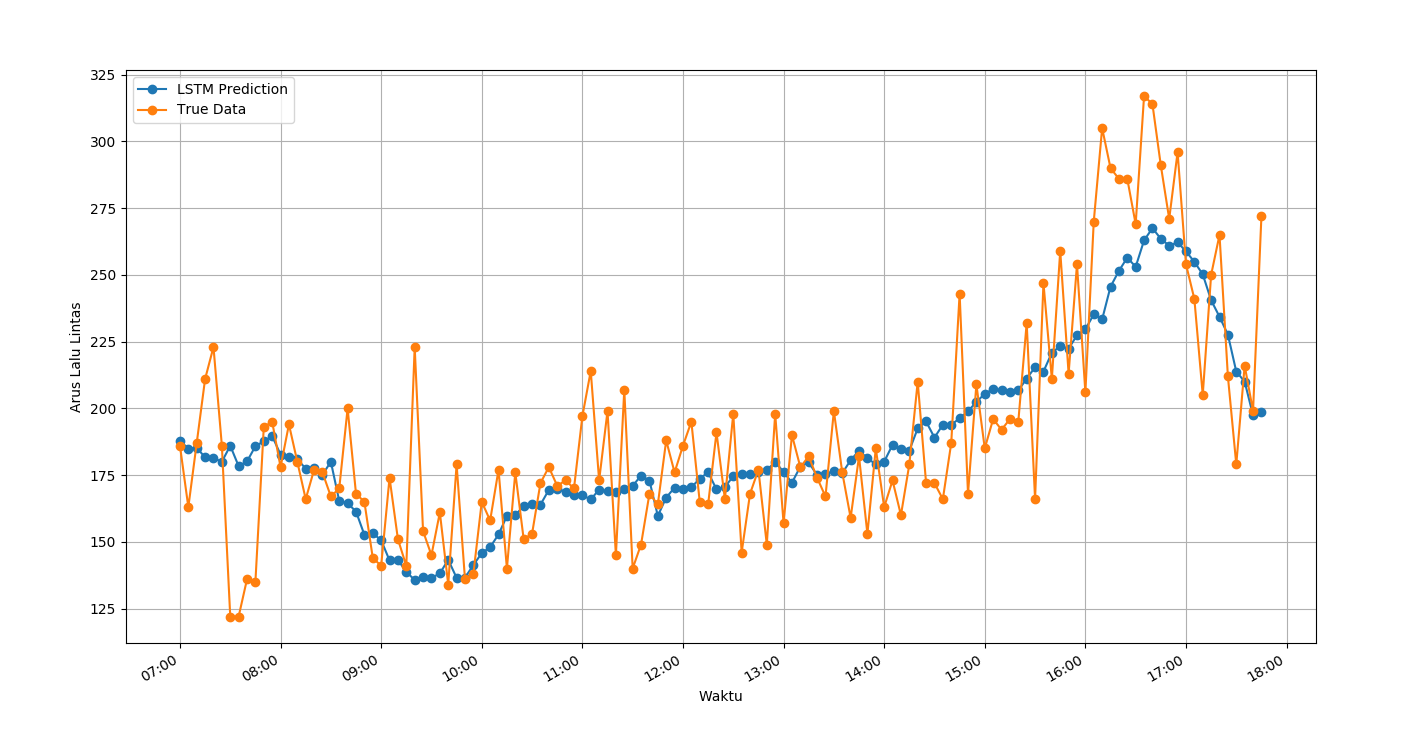
\includegraphics[scale=0.3]{out_130}
	\caption{Hasil prediksi model dengan output 130}
	\label{out_130}
\end{figure}

\begin{figure}[htp]
	\centering
	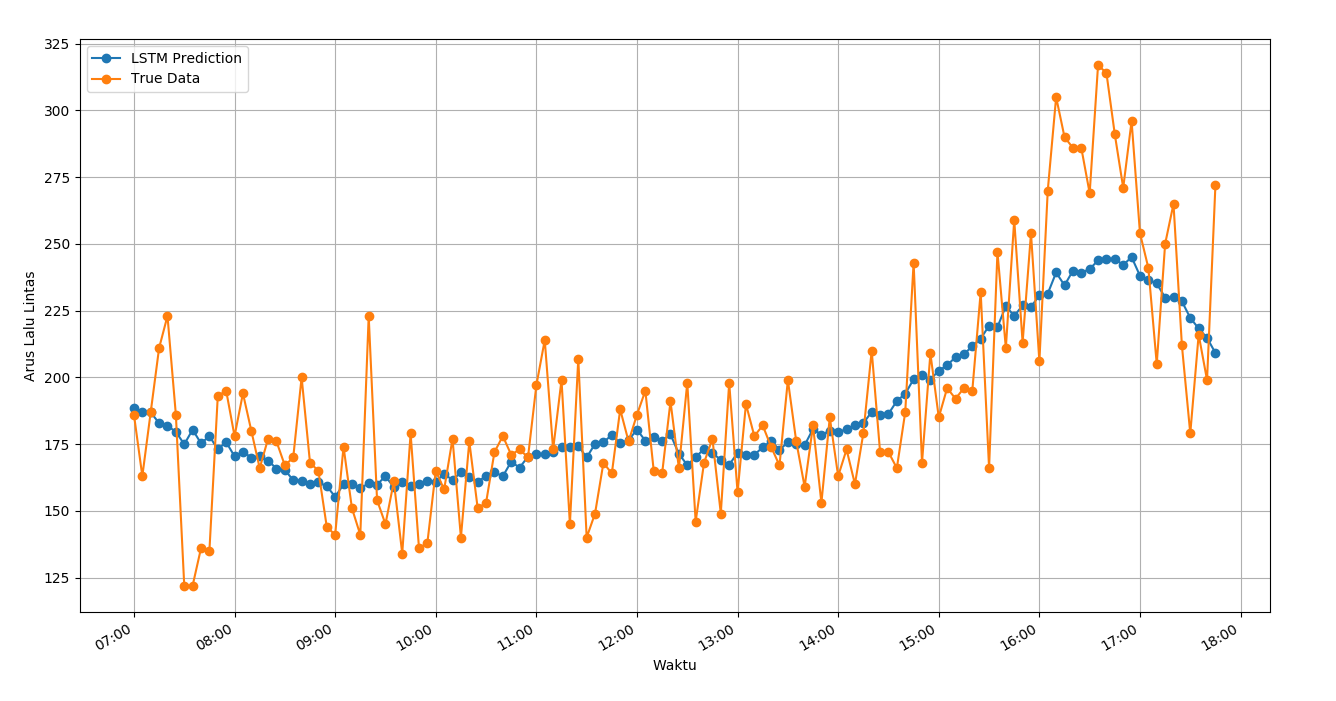
\includegraphics[scale=0.3]{out_65}
	\caption{Hasil prediksi model dengan output 65}
	\label{out_65}
\end{figure}

\begin{figure}[htp]
	\centering
	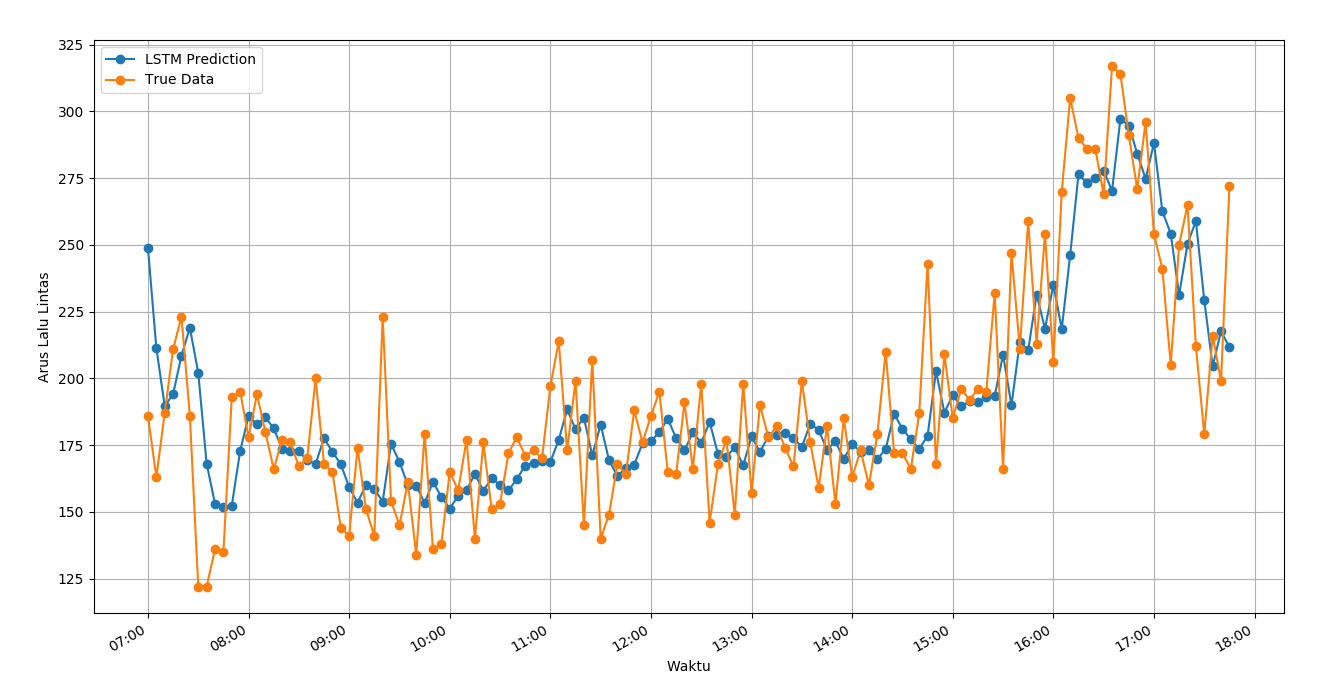
\includegraphics[scale=0.3]{out_1}
	\caption{Hasil prediksi model dengan output 1}
	\label{out_1}
\end{figure}
Berdasarkan gambar tersebut dapat diketahui bahwa meskipun nilai RMSE dan MAPE yang dimiliki oleh model dengan output 1 secara statistika lebih buruk daripada model dengan output 130 dan 65, namun secara visual model dengan output 1 mampu mengikuti tren dari data uji lebih baik. Hal ini dikarenakan dengan jumlah output yang semakin sedikit, maka model akan semakin presisi untuk mempelajari karakteristik data namun
akan membutuhkan waktu lama untuk melakukan prediksi. 

\section{Conclusion} \label{conclusion}

\emph{Kinodynamic motion planning} for omnidirectional mobile robot was presented in this work. Obstacles' motion and robot's dynamic was taken into account while planning the collision-free trajectory. Dynamic constraints for translational motion was addressed by 'soft' constraint via input control weight while 'hard' constraints for rotational motion was satisfied by setting maximum allowed velocity and acceleration. The presented sampling strategy was able to reduce solution cost. Online planning \& tracking scheme was presented. Dynamic simulation shows the scheme was successfully applied to the simulated robot and environment.

\bibliographystyle{IEEEtran}
\bibliography{reference}

\end{document}
